
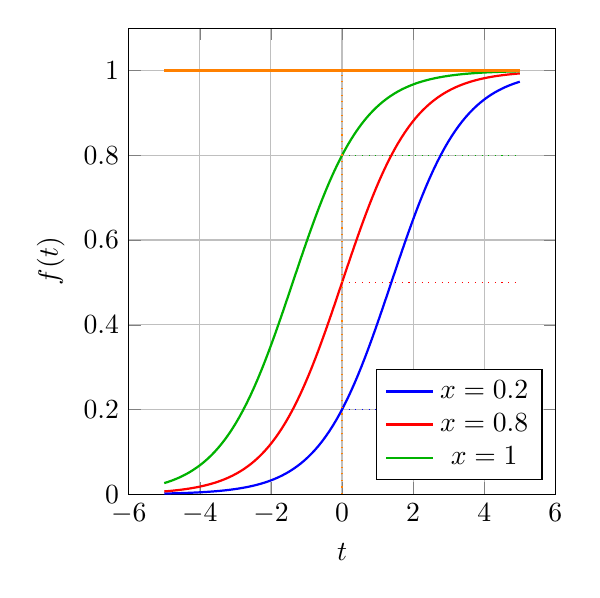
\begin{tikzpicture}[scale=1]
  \begin{axis}[
      domain==3:3,
      samples=100,
      xlabel={$t$},
      ylabel={$f(t)$},
      grid=major,
      ymin=0, ymax=1.1,
      legend pos=south east,
      width=7cm, height=7.5cm,
    ]

    % Values of x
    \def\xA{0.2}
    \def\xB{0.5}
    \def\xC{0.8}
    \def\xD{1}

    % Plot for x=0.2
    \addplot[blue, thick] {1/(1 + ((1/\xA)-1)*exp(-x))};
    \addlegendentry{$x=0.2$}
    % Dotted vertical line at t=0 from 0 to f(0)=x
    \draw[blue, dotted] (axis cs:0,0) -- (axis cs:0,\xA);
    % Dotted horizontal line at y=f(0)=x from t=0 to t=5
    \draw[blue, dotted] (axis cs:0,\xA) -- (axis cs:5,\xA);

    % Plot for x=0.5
    \addplot[red, thick] {1/(1 + ((1/\xB)-1)*exp(-x))};
    %\addlegendentry{$x=0.5$}
    \draw[red, dotted] (axis cs:0,0) -- (axis cs:0,\xB);
    \draw[red, dotted] (axis cs:0,\xB) -- (axis cs:5,\xB);

    % Plot for x=0.8
    \addplot[green!70!black, thick] {1/(1 + ((1/\xC)-1)*exp(-x))};
    \addlegendentry{$x=0.8$}
    \draw[green!70!black, dotted] (axis cs:0,0) -- (axis cs:0,\xC);
    \draw[green!70!black, dotted] (axis cs:0,\xC) -- (axis cs:5,\xC);

    % Plot for x=1
    \addplot[orange, thick] {1/(1 + ((1/\xD)-1)*exp(-x))};
    \addlegendentry{$x=1$}
    \draw[orange, dotted] (axis cs:0,0) -- (axis cs:0,\xD);
    \draw[orange, dotted] (axis cs:0,\xD) -- (axis cs:5,\xD);

  \end{axis}
\end{tikzpicture}
